\documentclass{article}

\usepackage{amsmath,amsfonts,amssymb,amsthm,mathtools,mathrsfs}
\usepackage[utf8]{inputenc}
\usepackage[T1]{fontenc}
\usepackage[english, russian]{babel}
\usepackage{fontspec}
\setmainfont[Ligatures={TeX,Historic}]{Times New Roman}


\title{HW01}
\author{Киреев Константин 8383}
\date{\today}

\newtheorem{problem}{Задача}

\begin{document}
\maketitle    
\renewcommand*{\proofname}{\textbf{Решение}}
    \begin{problem}
        Привести грамматику для языка $\{\alpha \cdot abbab \cdot \beta | \alpha, \beta \in \{a, b\}^*\}$. Привести вывод и дерево вывода для 2 различных цепочек из языка.
    \end{problem}
    \begin{proof}
        \begin{align*}            
            &G = \langle V_T, V_N, P, S \rangle \\
            &V_T = \{a, b\} \\
            &V_N = \{S, A, B\}
        \end{align*}
        \begin{align*}  
            P = \{&S\rightarrow A \\ 
            &A \rightarrow aA | abbabB \\
            &B \rightarrow bB | A | \epsilon \} 
        \end{align*}
        
        \begin{itemize}
            \item $aaabaab = S\rightarrow A \rightarrow aA\rightarrow aaA\rightarrow aaabbabB\rightarrow aaabbabbB\rightarrow aaabbabb\epsilon\rightarrow aaabbabb$
            \item $abbab = S\rightarrow A\rightarrow abbabB \rightarrow abbab\epsilon\rightarrow abbab$
        \end{itemize}
        \begin{figure}[h!]
            \center{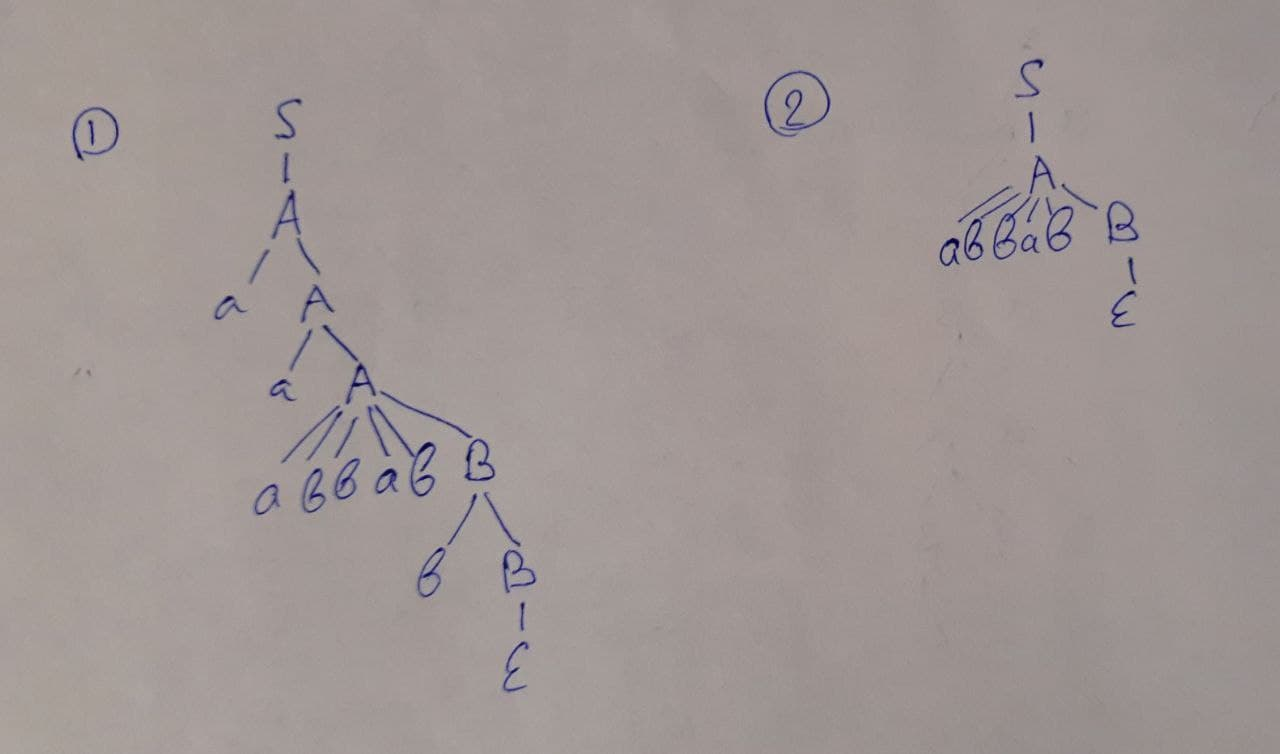
\includegraphics[scale=0.18]{1}}
        \end{figure}
    \end{proof}   
    \newpage
    \begin{problem}
        Доказать или опроыергнуть, что для любых языков $L$ и $M$ верно $(L\cdot M)^r = M^r \cdot L^r$
    \end{problem}
    \begin{proof}
        
    \end{proof}

    \begin{problem}
        Перечислить все слова языка $\{c^na^nt^n | n \in \mathbb{N}_0 \} \cap \{(cat)^m | m \in \mathbb{N}_0\}$
    \end{problem}
    \begin{proof}
        $ $
        \begin{itemize}
            \item cat
            \item $\epsilon$
        \end{itemize}
    \end{proof}
\end{document}